% flashcards-title: Vector subtraction construction
% flashcards-desc: Vector a is followed head-to-tail by minus b, while the original b direction is indicated separately.
\documentclass[border=7pt]{standalone}
\def\pgfsysdriver{pgfsys-dvisvgm.def}
\usepackage{tikz}
\usetikzlibrary{arrows.meta,positioning,shapes.geometric}
\definecolor{mechInk}{HTML}{172033}
\definecolor{mechBlue}{HTML}{155EEF}
\definecolor{mechOrange}{HTML}{B54708}
\definecolor{mechPale}{HTML}{E8F0FF}
\definecolor{mechGray}{HTML}{667085}
\definecolor{mechLight}{HTML}{D0D5DD}
\tikzset{
  every picture/.style={font=\sffamily\large, text=mechInk},
  mech box/.style={draw=mechInk, line width=1.2pt, rounded corners=4pt,
    fill=white, align=center, minimum height=14mm, inner xsep=5mm},
  mech primary/.style={draw=mechBlue, line width=2.2pt},
  mech secondary/.style={draw=mechOrange, line width=2.2pt, dashed},
  mech guide/.style={draw=mechGray, line width=0.9pt, dashed},
  mech arrow/.style={-{Stealth[length=3.2mm,width=2.4mm]},
    draw=mechInk, line width=1.4pt, line cap=butt},
  mech axis/.style={draw=mechInk, line width=1.2pt},
  mech tick/.style={draw=mechInk, line width=1pt}
}

\begin{document}
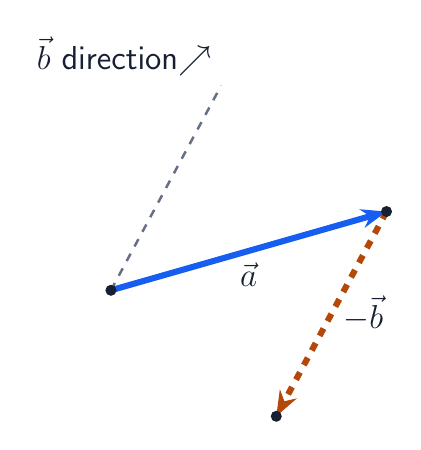
\begin{tikzpicture}[x=1cm,y=1cm]
  \coordinate (O) at (0,0); \coordinate (A) at (3.5,1); \coordinate (B) at (1.4,2.6); \coordinate (E) at (2.1,-1.6);
  \draw[mech guide] (O) -- (B);
  \draw[mech primary,-{Stealth[length=3.2mm,width=2.4mm]},line cap=butt] (O) -- (A) node[midway,below] {$\vec a$};
  \draw[mech secondary,-{Stealth[length=3.2mm,width=2.4mm]},line cap=butt] (A) -- (E) node[midway,right] {$-\vec b$};
  \node[above left] at (B) {$\vec b$ direction$\nearrow$};
  \fill[mechInk] (O) circle (2pt) (A) circle (2pt) (E) circle (2pt);
\end{tikzpicture}
\end{document}
